%!TEX root = thesis.tex

\chapter{Two topologically distinct smoothings}

Denote by $dP_6$ the del Pezzo surface of degree 6 embedded in $\PP^6$. This can be realized as the blow-up of $\PP^2$ in three points not lying on a line. Let $X$ denote the affine cone over $dP_6$. Then it has long been known that $X$ has two smoothing components, and we show here that they are topologically distinct.

Recall that a \emph{del Pezzo} surface is a surface such that the anti-canonical bundle is ample. The degree is the degree given by the anticanonical embedding. It is a classical result that every del Pezzo surface is obtained either by blowing up $\PP^2$ in $r=0,\ldots,6$ points in suitable positions, or as the $2$-uple embedding of a quadric surface in $\PP^3$. 

\section{Different embeddings of \texorpdfstring{$dP_6$}{dP6}}

We first obtain the equations of $dP_6$ directly from the description of it as blow-up. Let $x_0,x_1,x_2$ be coordinates of $\PP^2$. Recall that the blowup of $\PP^2$ in the point $(1:0:0)$ can be realized as the closed subscheme of $\PP^2 \times \PP^1$ given by the equation $r_0x_1-r_1x_2=0$, where $r_0,r_1$ are coordinates on $\PP^1$. We can repeat this process on the points $(0:1:0)$ and $(0:0:1)$ to obtain similar equations. Collecting these, we see that $dP_6$ is given by the matrix equation
\[
M\vec x = 
\begin{pmatrix}
0 & r_0 & -r_1 \\
s_1 & 0 & -s_0 \\
-t_0 & t_1 & 0
\end{pmatrix}
\begin{pmatrix}
x_0 \\ y_0 \\ z_0
\end{pmatrix}= 0.
\]
in $\PP^2 \times \PP^1 \times \PP^1 \times \PP^1$. Here $r_i,s_i$ and $t_i$ ($i=0,1$) are of course coordinates on $\PP^1$.

We can do more than this however. 

\begin{lemma}
We can also realize $dP_6$ embedded in $\PP^1 \times \PP^1 \times \PP^1$ with equation $r_0s_0t_0=r_1s_1t_1$.
\end{lemma}
\begin{proof}
Note that the matrix cannot have rank $1$ or lower. Now consider the projection onto the last three factors:
$$
\pi:\PP^2 \times \PP^1 \times \PP^1 \times \PP^1 \to \PP^1 \times \PP^1 \times \PP^1.
$$
Each point $P$ in the product on the right-hand side gives a matrix $M_P$ of rank $2$. Thus there is a line of solutions, which correspond exactly to a point in $\PP^2$.

Hence the restriction of $\pi$ to $dP_6$ is an isomorphism onto the hypersurface given by $\det M=0$ in $\PP^1 \times \PP^1 \times \PP^1$. 
\end{proof}

Another way to realize blow-ups is this: let $\mathfrak d$ be the linear system of quadrics with assigned basepoints $(1:0:0)$, $(0:1:0)$ and $(0:0:1)$ in $\PP^2$. We can choose a basis given by $x_0x_1,x_0x_2$ and $x_1x_2$. This gives a rational map $\PP^2 \rmap \PP^2$. The closure of the graph of this map is a subvariety of $\PP^2 \times \PP^2$ defined by two bilinear equations. Each of the projections correspond to the blowup.

Explicitly, if we let $y_0,y_1,y_2$ be coordinates on the other $\PP^2$, then the equations are $x_1y_0-x_1y_1=x_1y_1-x_2y_2=0$.

We also have a natural embedding in $\PP^6$ as follows. Denote by $E_1, E_2, E_3$ the exceptional divisors on the blowup. Let $L$ be a line in $\PP^2$. Then the divisor $\pi^\ast 3L - E_1-E_2-E_3$ is ample, and gives an embedding in $\PP^6$ (see \cite[Chapter V, Theorem 4.6]{hartshorne}). A basis for the corresponding linear system is given by all monomials in $\Gamma(\PP^2,\OO_{\PP^2}(3))$ except $x^3,y^3$ and $z^3$. 

The equations can be arranged in a particularly symmetric form: let $y,x_1,\ldots,x_1$ be coordinates on $\PP^6$. Then the equations of $dP_6$ are the $2 \times 2$ minors of the matrix
$$
\begin{pmatrix}
x_1 & y & x_6 \\
x_2 & x_3 & y \\
y & x_4 & x_5
\end{pmatrix}.
$$
This gives $9$ equations, which can be compactly written as $x_ix_{i+2}-yx_i=0$ and $x_ix_{i+3}-y^2=0$, for $i=1,\ldots,6$ (where $i$ is taken modulo $6$). Note that the equations have a visible $D_6$-symmetry, where $D_6$ denotes the dihedral group.

\subsection{As a toric variety}

There is a nice combinatorial description of $dP_6$ as a toric variety associated to a polytope. Namely, let $P$ denote the hexagon in \figref{hexagon}. Then the normal fan of this polytope defines a fan in $N_\R$, defining a toric variety.

\begin{figure}
\centering
\begin{subfigure}{.4 \textwidth}
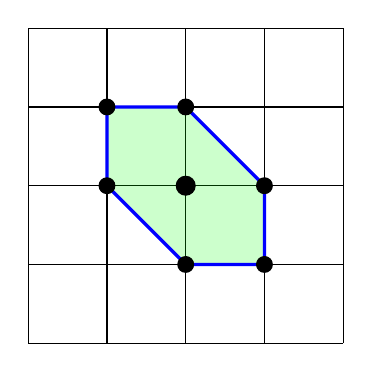
\begin{tikzpicture}
  \draw (0, 0) grid (4, 4);  

\draw [very thick, color=blue, fill=green, fill opacity=0.2]
(2,1) -- (3,1) -- (3,2) -- (2,3) -- (1,3) -- (1,2) -- cycle;

\draw [fill=black]  (2, 1) circle (0.1);
\draw [fill=black]  (3, 1) circle (0.1);
\draw [fill=black]  (3, 2) circle (0.1);
\draw [fill=black]  (2, 3) circle (0.1);
\draw [fill=black]  (1, 3) circle (0.1);
\draw [fill=black]  (1, 2) circle (0.1);
\draw [fill=black]  (2, 2) circle (0.12);
\end{tikzpicture}
\caption{The hexagon.}
\label{fig:hexagon}
\end{subfigure}
\begin{subfigure}{.4 \textwidth}
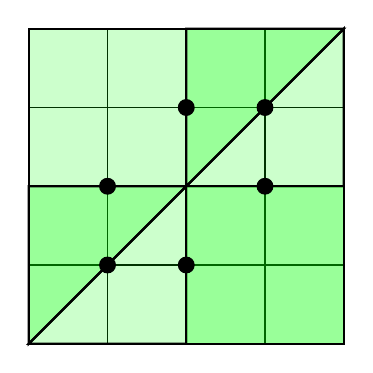
\begin{tikzpicture}
  \draw (0, 0) grid (4, 4);  
%\draw [very thick, fill=green, fill opacity=0.2]
%(1,1) -- (2,1) -- (3,2) -- (3,3) -- (2,3) -- (1,2) -- cycle;
\draw [thick,fill=green, fill opacity=0.2] (2,2) -- (4,2) -- (4,4) -- cycle;
\draw [thick,fill=green, fill opacity=0.4] (2,2) -- (4,4) -- (2,4) -- cycle;
\draw [thick,fill=green, fill opacity=0.2] (2,2) -- (2,4) -- (0,4) -- (0,2) -- cycle;
\draw [thick,fill=green, fill opacity=0.4] (2,2) -- (0,2) -- (0,0) -- cycle;
\draw [thick,fill=green, fill opacity=0.2] (2,2) -- (0,0) -- (2,0) -- cycle;
\draw [thick,fill=green, fill opacity=0.4] (2,2) -- (2,0) -- (4,0) -- (4,2) -- cycle;

\draw [fill=black]  (1, 1) circle (0.1);
\draw [fill=black]  (2, 1) circle (0.1);
\draw [fill=black]  (3, 2) circle (0.1);
\draw [fill=black]  (3, 3) circle (0.1);
\draw [fill=black]  (2, 3) circle (0.1);
\draw [fill=black]  (1, 2) circle (0.1);
%\draw [fill=black]  (2, 2) circle (0.1);
\end{tikzpicture}
\caption{The fan of $dP_6$.}
\label{fig:fandp6}
\end{subfigure}
\caption{Toric description of $dP_6$.}
\end{figure}

The polytope is reflexive, implying that the normal fan of $P$ is the face fan over the same polytope. See \figref{fandp6}. From standard toric geometry, it is clear that $dP_6$ is the blowup of $\PP^2$ in the three torus-fixed points. 

\section{Divisors and topology}

Consider the exponential sequence
\[
0 \to \Z \to \OO_{dP_6} \to \OO_{dP_6}^\ast \to 0.
\]

Since $dP_6$ is a rational surface, it follows from the long-exact sequence that $H^2(dP_6,\Z) \simeq \Pic(dP_6)$. From the description of $dP_6$ as a blowup, we know from \cite[Chapter V]{hartshorne}, that the Picard group is spanned by the three exceptional divisors, together with the class of the pullback of a hyperplane. 

%% Picard group
%% cohomology groups

\section{The affine cone and its two smoothings}

Let $X$ denote the affine cone over $dP_6$. It is an affine variety with an isolated singularity at the origin. One can compute that it has two smoothing components: the union of a plane and a line. They both come from different ways of perturbing the equations of $dP_6$.

\begin{figure}
\centering 
\begin{subfigure}{.4 \textwidth}
  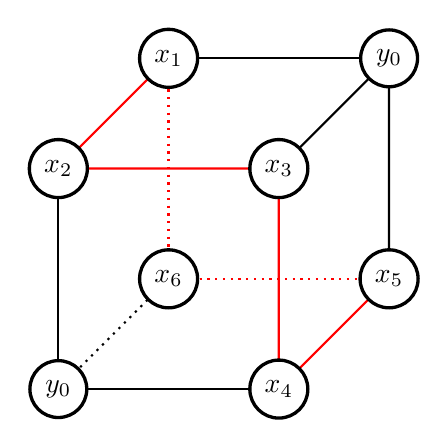
\begin{tikzpicture}[scale=1.4,every node/.style={circle, draw=black, fill=white}, every path/.style={very thick}]
\coordinate (A) at (0,0);
\coordinate (B) at (2,0);
\coordinate (C) at (2,2);	
\coordinate (D) at (0,2);	
\coordinate (E) at (1,1);	
\coordinate (F) at (3,1);	
\coordinate (G) at (3,3);	
\coordinate (H) at (1,3);	
\draw[thick, color=red] (D)  -- (C) -- (B) --(F);  %1
\draw[thick, color=red, dotted] (H) -- (E);
\draw[thick, color=red, dotted] (E) -- (F);
\draw[thick, color=red] (D) -- (H);
\draw[thick] (D) -- (A) -- (B);
\draw[thick] (C) -- (G) -- (F);
\draw[thick] (H) -- (G);
\draw[thick, dotted] (A) -- (E);

\draw (A) node {$y_0$};
\draw (B) node {$x_4$};
\draw (C) node {$x_3$};
\draw (D) node {$x_2$};
\draw (E) node {$x_6$};
\draw (F) node {$x_5$};
\draw (G) node {$y_0$};
\draw (H) node {$x_1$};
\end{tikzpicture}
  \caption{Equations $dP_6$.}
  \label{fig:dp6p1}
 \end{subfigure}
\begin{subfigure}{.4\textwidth}
  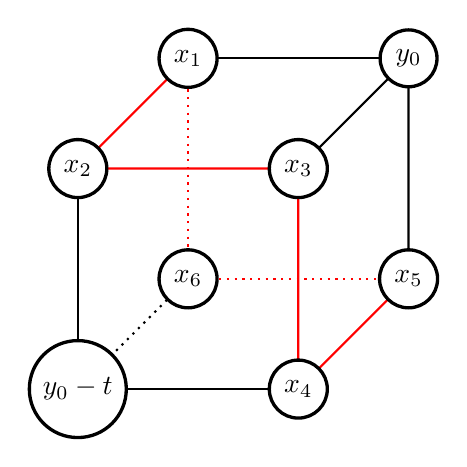
\begin{tikzpicture}[scale=1.4,every node/.style={circle, draw=black, fill=white}, every path/.style={very thick}]
\coordinate (A) at (0,0);
\coordinate (B) at (2,0);
\coordinate (C) at (2,2);	
\coordinate (D) at (0,2);	
\coordinate (E) at (1,1);	
\coordinate (F) at (3,1);	
\coordinate (G) at (3,3);	
\coordinate (H) at (1,3);	

\draw[thick, color=red] (D)  -- (C) -- (B) --(F);  %1
\draw[thick, color=red, dotted] (H) -- (E);
\draw[thick, color=red, dotted] (E) -- (F);
\draw[thick, color=red] (D) -- (H);
\draw[thick] (D) -- (A) -- (B);
\draw[thick] (C) -- (G) -- (F);
\draw[thick] (H) -- (G);
\draw[thick, dotted] (A) -- (E);

\draw (A) node {$y_0-t$};
\draw (B) node {$x_4$};
\draw (C) node {$x_3$};
\draw (D) node {$x_2$};
\draw (E) node {$x_6$};
\draw (F) node {$x_5$};
\draw (G) node {$y_0$};
\draw (H) node {$x_1$};
\end{tikzpicture}
  \caption{Deforming $C(dP_6)$.}
  \label{fig:dp6p12}
  \end{subfigure}
 \caption{Forms of equations.}
\end{figure}

Look at \figref{dp6p1}. One can read off the equations of $dP_6$ by taking minors along ``faces'' and long diagonals of this square. This correspond to a hyperplane cut of $\PP^ 1 \times \PP^1 \times \PP^1$ in the Segre embedding. Then the one-dimensional component of the versal deformation of $X$ is obtained by perturbing one of the $y_0$-corners as in \figref{dp6p12}.

It is clear the corresponding deformation is smooth, since it is a hyperplane cut of cone over $\PP^1 \times \PP^1 \times \PP^1$ outside the origin. Call this smoothing $X_1$.

\begin{lemma}
The smoothing $X_1$ is isomorphic to $\PP^1 \times \PP^1 \times \PP^1 \bs dP_6$.
\end{lemma}
\begin{proof}
Specialize to some $t \neq 0$. Then we can homogenize the equations with respect to $y_1$ to obtain a projective variety in $8$ variables. However, in this form, $y_0-ty_1$ and $y_0$ are linearly independent, hence by a change of variables, we see that this variety is in fact isomorphic to $\PP^1 \times \PP^1 \times \PP^1$ in its Segre embedding. See \figref{dp6p12}.

What we gained by homogenizing is exactly the projective variety given by setting $y_1=0$. But then we get back the equations of $dP_6$ in $\PP^6$.
\end{proof}

The second smoothing is obtained by deforming the equations of $dP_6$ as a subvariety of $\PP^2 \times \PP^2$. Namely, consider the following matrix:

\begin{equation}
\label{eq:def2}
\begin{vmatrix}
x_1 & y_0 & x_6 \\
x_2 & x_3 & y_0-t_1 \\
y_0-t_2 & x_4 & x_5
\end{vmatrix} \leq 1.
\end{equation}


For $t_1=t_2=0$, we get the cone over $dP_6$, while for generic $t_i$, we get a smooth variety. In fact, we can compute that the discrimant locus (the set of points in $\Aa^2_{t_1,t_2}$ with singular fiber) are the $t_1$-axis, the $t_2$-axis and the line $t_1=t_2$. 

Call (any) smooth fiber $X_2$. 

\begin{lemma}
Let $M=\PP(\mathcal T_ {\PP^2})$ be the projective bundle associated to the tangent sheaf on $\PP^2$. Then the smoothing $X_2$ is isomorphic to $M \bs dP_6$. 
\end{lemma}
\begin{proof}
The technique is the same as in the previous proof. First homogenize the equations \eqref{eq:def2} with respect to $y_1$. Call the homogenized variety $M$. Put $y_0'=y_0$, $y_1' = y_0-ty_1$ and $y_2'=y_0-t_2y_1$. Then we have the relation
\[
h = t_2y_1'-t_1y_2' - (t_1-t_2)y_0' = 0.
\]
Hence we see that $M=\PP^2 \times \PP^2 \cap (h = 0)$. We can pull back the coordinates $y_i'$ to $\PP^2 \times \PP^2$. Let $\PP^2 \times \PP^2$ have coordinates $x_0,x_1,x_2$ and $y_0,y_1,y_2$. Then $h$ pulls back to the equation
\[
(x_0,x_1,x_2) \cdot (-t_1y_2, (t_1-t_2)y_0,t_2y_1) = 0
\]
in $\PP^2 \times \PP^2$. As long as $t_1 \neq t_2$ and $t_1,t_2 \neq 0$, we can do a change of coordinates in $\PP^2_{y_0y_1y_2}$, so that $h$ transforms to
\[
(x_0,x_1,x_2) \cdot(y_0,y_1,y_2) = 0.
\]
Hence we see that $M$ is isomorphic to the total space of the Grassmannian of lines in $\PP^2$ (each point in one of the $\PP^2$'s give a line in the other $\PP^2$). This is in turn isomorphic to $\PP(\mathcal T_{\PP^2})$, since each tangent vector through a point determines a line through it.

Now, what have we gained by homogenizing? The divisor at infinity is $y_1=0$, which is a $dP_6$ again. In our new coordinates this is equivalent to $y_1'=y_2'=y_0'$. Hence in the coordinates of $\PP^2 \times \PP^2$, the $dP_6$ is given by the two equations $x_1y_0-x_2y_1=x_1y_0-x_0y_2=0$. 
\end{proof}

\begin{lemma}
The cohomology ring of $M=\PP(\mathcal T_{\PP^2})$ is $\Z[x,y]/(x^3,y^2+c_1(E)y+c_2(E))$. In particular, the cohomology of $M$ is given by $(1,0,2,0,2,0,1)$.
\end{lemma}
\begin{proof}
This is a consequence of the Leray-Hirsch theorem. See \cite{bott_tu} for a proof.
\end{proof}

We can use what we know about the topology of these spaces to compute homology groups of the two affine smoothings.

\begin{thm}
The two affine smoothings are topologically different. The homology groups are:
\begin{center}
\begin{tabular}{ l || c | c | c | c | c | c | c || c }
 Group & 0 & 1 & 2 & 3 & 4 & 5 & 6 & Euler-characteristic \\
\hline
$H^i(X_1,\Z)$ & 1 & 0 & 2 & 1 & 0 & 0 & 0 & 2 \\
$H^i(X_2,\Z)$ & 1 & 0 & 1 & 2 & 0 & 0 & 0  & 0
\end{tabular}
\end{center}
\end{thm}

\begin{proof}
The singular cohomology of $M=\PP^1 \times \PP^1 \times \PP^1$ is given by $(1,0,3,0,3,0,1)$, which can be computed by the Künneth formula. The cohomology of $dP_6$ is given by $(1,0,4,0,1)$.

We will use the Lefschetz duality theorem \cite{spanier_topology}, which in this case says that $H_q(M \bs dP_6, \Z) \simeq H^{6-q}(M,dP_6,\Z)$. Then the long exact sequence of the pair $(M,dP_6)$ immediately gives $h_0(X_1,\Z)=1$. Similarly, we see that $h_5(X_1,\Z)=h_6(X_1,\Z)=0$, since the map $H^1(M,\Z) \to H^1(D,\Z)$ is an isomorphism.

The other groups depend upon the explicit form of the maps $H^2(M,\Z) \to H^2(D,\Z)$ and $H^4(M,\Z) \to H^4(D,\Z)$.

By Poincaré duality ((reference)), the induced map corresponds to intersecting the divisors on $M$ with $dP_6$. Computing, we get that map is given by the following matrix:
\[
H^2(M,\Z) \simeq H_4(M,\Z) \simeq \Z^3 \xrightarrow{
	\begin{pmatrix}
	0 & 1 & 1 \\
	1 & 0 & 1 \\
	1 & 1 & 0 \\
	0 & 0 & 0
	\end{pmatrix}
} \Z^4 \simeq H_2(dP_6,\Z) \simeq H^2(dP_6,\Z).
\]

This is an injective map, and it follows from the long-exact sequence and the Lefschetz theorem that $H_3(X_1) \simeq H^3(M,dP_6) \simeq \Z$, and also that $H_4(X_1)=0$.

Similarly, the map $H^4(M) \to H^4(dP_6)$ is computed to be given by $(a,b,c) \mapsto a+b+c$, since the three $\PP^1$'s intersect $dP_6$ in a single point. This map has two-dimensional kernel, and we conclude that $H_2(X_1) \simeq H^4(M,dP_6) = \Z^2$, and that $H^1(X_1)=0$.

The computations for $X_2$ are similar but more involved. We first 


%%% (X_2)tillukning er PP(PP_2), evt totalrommet til Grassmannian Gr(1,P^2).
%%% Denne har kohomologi lik P^2 \times P^1.
%%% Beregn avbildningene.
\end{proof}

\begin{remark}
In fact, the Andreotti-Frankel theorem \cite{andreotti_affinecw} states the following: if $V$ is any smooth affine variety of complex dimension $n$, then it has the homotopy type of a CW complex of dimension $n$.
\end{remark}